
\noindent
\begin{tabular}{cc}
\begin{minipage}{0.60\textwidth}
%\sectionIf{\flagSect}{\taitol{Esercizio}}
\begin{exercise}[Azioni statiche: diga]
Si consideri la sezione di diga rappresentata in figura.
Si determini il modulo e la direzione del risultante 
delle forze per unit\`a di apertura agente sui diversi 
tratti rettilinei della diga stessa sapendo che la pressione
atmosferica \`e di $1.01 \times 10^5\ Pa$. Dimensioni: $a=10\ m$,
$b=2\, m$, $c=8\ m$, $d=10\ m$, $e=5\ m$, $f=3\ m$.\\ 
($\bm{R}_1=347100\hat{\bm{x}}\  N/m$,   \\
 $\quad \bm{R}_2=- 1043200\hat{\bm{z}}\ N/m$, \\
 \quad $\bm{R}_3=774500\hat{\bm{x}}\ N/m$,    \\
 \quad $\bm{R}_4=2284000 N/m \bm{\hat{x}} + 2284000 N/m \bm{\hat{z}}$,  \\
 \quad $\bm{R}_5=2774000\hat{\bm{z}}\ N/m$.)
\end{exercise}
\end{minipage}
&
\begin{minipage}{0.35\textwidth}
   \begin{center}
   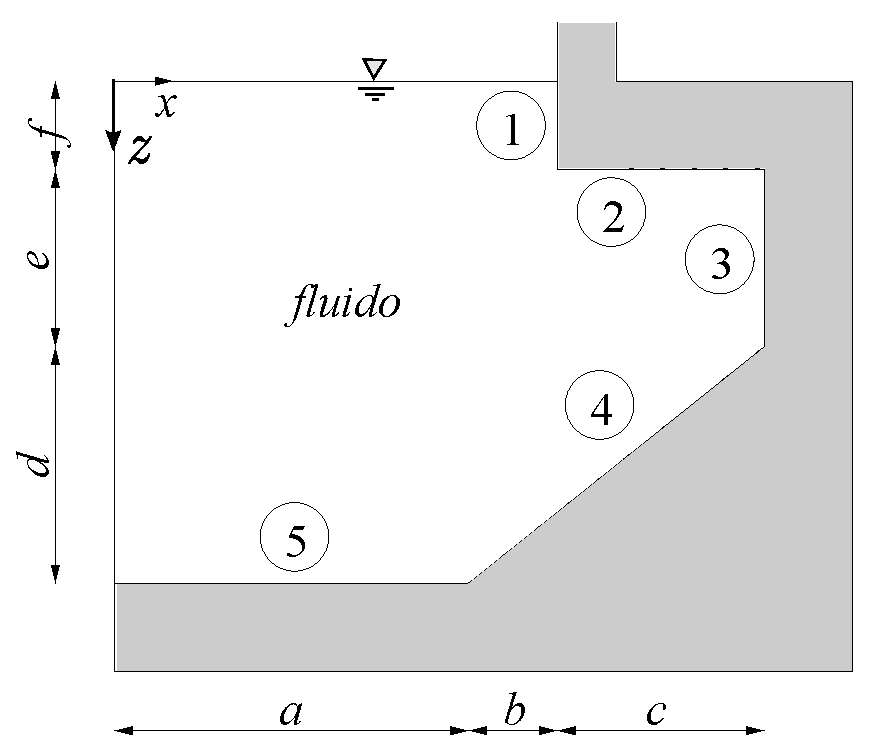
\includegraphics[width=0.90\textwidth]{./fig/diga2.eps}
   \end{center}
\end{minipage}
\end{tabular}


\sol

\partone
Legge di Stevino, $P_1 + \rho g h_1 = P_2 + \rho g h_2$.
%
 Calcolo della risultante delle azioni statiche, data la distribuzione di pressione e la normale $\bm{\hat{n}}$ uscente dal volume fluido,
\begin{equation}
   \bm{R} = \int_{S} P \bm{\hat{n}} \ .
\end{equation}

\parttwo
 Si risolve il problema bidimensionale, al quale ``manca'' la dimensione perpendicolare al piano del disegno. La risultante per unità di apertura agente sul lato $\ell$ (unità di misura nel SI, $N/m$) sarà quindi il risultato dell'integrale di linea
\begin{equation}
   \bm{R} = \int_{\ell} P \bm{\hat{n}} \ .
\end{equation} 
 Per ogni lato si calcola la distribuzione di pressione, grazie alla legge di Stevino. Si integra la distribuzione di pressione per ottenere il modulo della risultante; la direzione coincide con quella della normale (uscente dal volume occupato dal fluido).
Per lo svolgimento, è stato scelto il sistema di riferimento rappresentato in figura, con l'asse x diretto verso destra e l'asse z verso il basso.

\begin{itemize}

 \item Lato 1. Pressione lineare in z, $P(z) = P_O + \rho g z , \ z \in [0,f] $. Risultante
   \begin{equation}
   \bm{R}_1 = \int_{\ell_1} P \bm{\hat{n}} = \int_{0}^{f} (P_O + \rho g z) \bm{\hat{x}} dz = 
     \displaystyle\left(P_O  f + \frac{1}{2} \rho g f^2 \right) \bm{\hat{x}} = 347100 N/m \bm{\hat{x}}
   \end{equation}
 \item Lato 2. Pressione costante, $P = P_O + \rho g f$. Risultante 
   \begin{equation}
     \bm{R}_2 = \int_{\ell_2} P \bm{\hat{n}} = P\cdot c (-\bm{\hat{z}})=(P_O + \rho g f)\cdot c(-\bm{\hat{z}}) = - 1043200 N/m \bm{\hat{z}}
   \end{equation}
 \item Lato 3. Pressione lineare in z, $P(z) = P_O + \rho g z , \  z \in [f,f+e]$. Risultante
   \begin{equation}
     \bm{R}_3 = \int_{\ell_3} P \bm{\hat{n}} = \int_{f}^{f+e} (P_O + \rho g z) \bm{\hat{x}} dz = 
     \displaystyle\left(P_O e + \frac{1}{2} \rho g \left[(f+e)^2 - f^2\right]\right) \bm{\hat{x}} = 774500 N/m \bm{\hat{x}}
   \end{equation}
 \item Lato 4. Pressione lineare in z, $P(z)  = P_O + \rho g z , \ z \in [f+e,f+e+d]$. Poichè il tratto di parete è rettilineo, il vettore normale è costante e può essere portato fuori dall'integrale. Si calcola prima il modulo della risultante e poi lo si moltiplica per il versore normale. Il modulo della risultante vale
   \begin{equation}
   \begin{aligned}
      {R}_4 & = \int_{\ell_4} P d\ell = \int_{f+e}^{f+e+d} P(z) \frac{\sqrt{(b+c)^2+d^2}}{d} dz = \qquad \qquad \text{$\displaystyle\left(d\ell = \frac{\sqrt{(b+c)^2+d^2}}{d} dz \right)$} \\
     & = \int_{f+e}^{f+e+d} (P_O + \rho g z) \frac{\sqrt{(b+c)^2+d^2}}{d} dz = \\
     & = \frac{\sqrt{(b+c)^2+d^2}}{d}\left[ P_O d + \frac{1}{2} \rho g \left((f+e+d)^2-(f+e)^2 \right)  \right] = 
     \sqrt{2} \cdot 2284000 N/m \\
   \end{aligned}
   \end{equation}
   La forza può essere scritta come $\bm{R}_4 = R_4 \bm{\hat{n}}_4$, con
   $\bm{\hat{n}}_4 = 1/\sqrt{2} \ \hat{\bm{x}} + 1/\sqrt{2} \ \hat{\bm{z}}$. Proietttando $\bm{R}_4$ lungo gli assi si ottengono le componenti orizzontali
   e verticali
   \begin{equation}
     \bm{R}_4 = 2284000 N/m \bm{\hat{x}} + 2284000 N/m \bm{\hat{z}}
   \end{equation}
 \item Lato 5. Pressione costante, $P = P_O + \rho g (f+e+d)$. Risultante 
   \begin{equation}
     \bm{R}_5 = P\cdot a \bm{\hat{z}} =(P_O + \rho g (f+e+d))\cdot a \bm{\hat{z}} =  2774000 N/m \bm{\hat{z}}
   \end{equation}
 
\end{itemize}

